%************************************************
\chapter{Basic Concepts}\label{ch:introductionplanning}
%************************************************
General Introduction to Thesis

\section{Classic Path Planning Problem}\label{sec:basic}

\section{Representation of the Environment}\label{sec:representation}
Exact Cell Decomposition
Approximate Cell Decomposition
Visibility Graph
Voronoi Regions

\section{Robotic Models}\label{sec:model}
Overview and classification of path planning algorithms

\section{Planning}\label{sec:global}
Global Planning:
Breadth-First Search (BFS)
Depth-First Search (DFS)
Dijkstra's and A* algorithm
An illustration is given in Figure~\ref{fig:fig_overview}
\begin{figure}[thpb]
	  \myfloatalign
      \footnotesize
      \centering
    \subfloat[Dijkstra algorithm]
    {  \label{fig:fig_djikstra}
        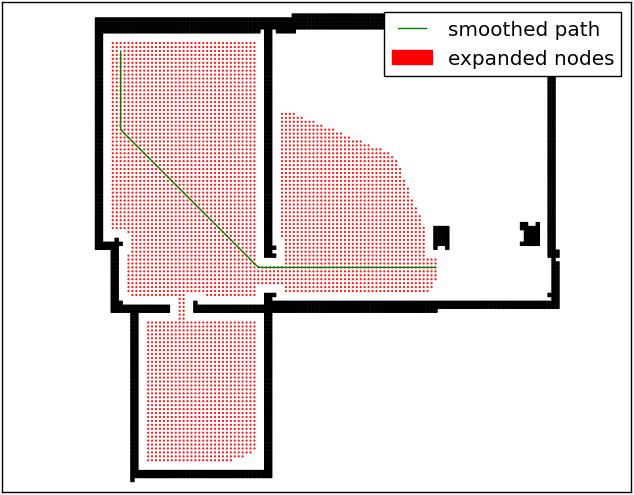
\includegraphics[width=0.75\textwidth]{figures/fig_djikstra.png}
        %\caption{Dijkstra}
    }
    
    \subfloat[A* algorithm]
    {  \label{fig:fig_astar}
       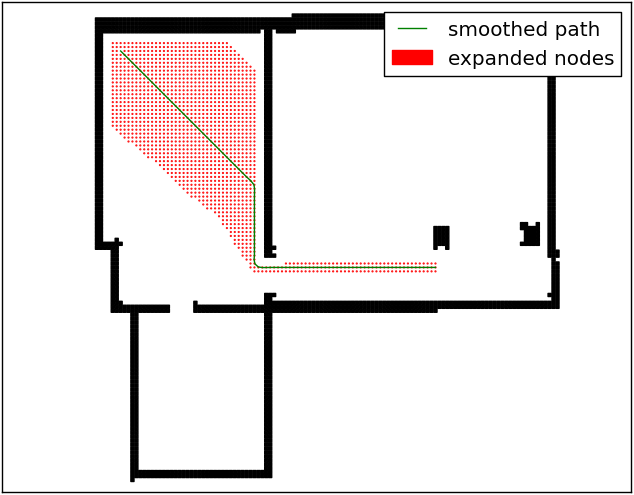
\includegraphics[width=0.75\textwidth]{figures/fig_astar.png}
       %\caption{A*}
    }
   \caption[Djikstra's and A* algorithm.]{The difference between Djikstra's and A* algorithm searching for a shortest path in a grid representation of a building. A* is more effective, as it visits by far less nodes in the search graph. }
\label{fig:fig_overview}
\end{figure}
Examples: 
Rapidly Exploring Randomized Trees (RRT)
Probabilistic Road Maps (PRM)
Potential Field

Local Planning:
The next chapter investigates local planning methods.

%*****************************************
%*****************************************
%*****************************************
%*****************************************
%*****************************************




